% Marius-Juston 2026
\documentclass[border=0pt]{standalone}
\usepackage{tikz}
\usetikzlibrary{arrows.meta, 3d}

\begin{document}
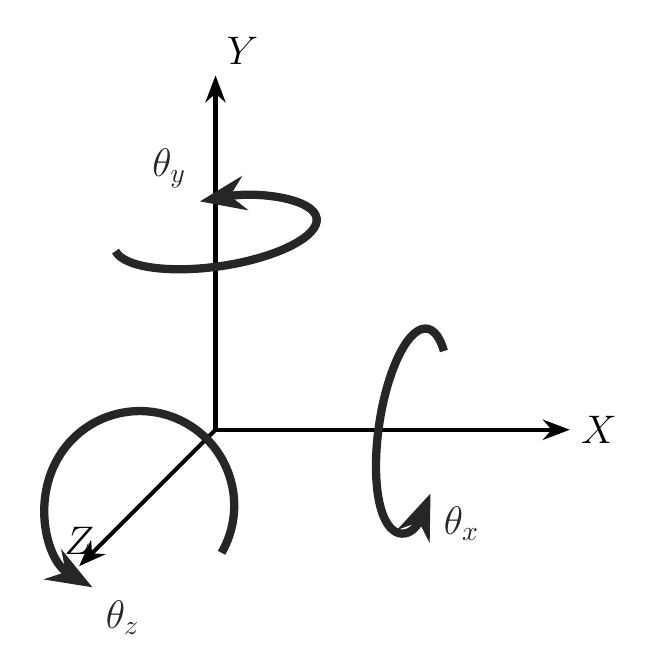
\begin{tikzpicture}[
    >=Stealth,
    axis/.style={->, line width=1.5pt},
    rot/.style={->, line width=3pt, color=black!85}
]

% Define lengths and parameters
\def\L{4.5}     % Length of translation axes
\def\R{1.2}     % Radius of rotation arcs
\def\pos{2.5}   % Position of the arc along the axis

% --- TRANSLATIONAL DOF (Axes) ---
\draw[axis] (0,0,0) -- (\L,0,0) node[right, font=\Large] {$X$};
\draw[axis] (0,0,0) -- (0,\L,0) node[above right, font=\Large] {$Y$};
\draw[axis] (0,0,0) -- (0,0,\L) node[above, font=\Large] {$Z$};

% --- ROTATIONAL DOF (Arcs) ---

% \theta_x around the X-axis
% Drawn exclusively in the local YZ plane translated along X
\begin{scope}[canvas is yz plane at x=\pos]
    \draw[rot] (-60:\R) arc (-60:210:\R) node[anchor=north west, font=\Large] {$\theta_x$};
\end{scope}

% \theta_y around the Y-axis
% Drawn exclusively in the local ZX plane translated along Y
\begin{scope}[canvas is zx plane at y=\pos]
    \draw[rot] (-60:\R) arc (-60:210:\R) node[anchor=south east, font=\Large] {$\theta_y$};
\end{scope}

% \theta_z around the Z-axis
% Drawn exclusively in the local XY plane translated along Z
\begin{scope}[canvas is xy plane at z=\pos]
    \draw[rot] (-30:\R) arc (-30:240:\R) node[anchor=north west, font=\Large] {$\theta_z$};
\end{scope}

\end{tikzpicture}
\end{document}